\documentclass[a4paper,12pt,Times]{article}
\usepackage{abakos}  %pacote com padrão da Abakos baseado no padrão da PUC
\usepackage{multirow}
\usepackage{tabularx}
\usepackage{float}
\usepackage{abntex2cite}
\usepackage{graphicx}
\usepackage{caption}
\usepackage{subcaption}

% https://norwied.wordpress.com/2012/07/10/how-to-break-long-urls-in-bibtex/
\usepackage{url}
\usepackage{breakurl}
%\usepackage[breaklinks]{hyperref}

\def\UrlBreaks{\do\/\do-}
%%%%%%%%%%%%%%%%%%%%%%%%%%%
%Capa da revista
%%%%%%%%%%%%%%%%%%%%%%%%%%

%\setcounter{page}{80} %iniciar contador de pagina de valor especificado
\newcommand{\monog}{Aprendizado por Reforço em Veículos Autônomos para Detecção de Faixas em Condições de Baixa Visibilidade}
\newcommand{\monogES}{Reinforcement Learning in Autonomous Vehicles for Lane End Detection in Low Visibility Conditions}
\newcommand{\tipo}{Artigo }  % Especificar a seção tipo do trabalho: Artigo, Resumo, Tese, Dociê etc
\newcommand{\origem}{Brasil}
\newcommand{\editorial}{\textbf{Abakos}, Belo Horizonte,v. 1, n. 1, p. 00-00, Jul. 2013 - ISSN: 2316-9451}  % p. xx-xx – páginas inicial-final do artigo
% \newcommand{\lcc}{\scriptsize{Licença Creative Commons Attribution-NonCommercial-NoDerivs 3.0 Unported}}

%%%%%%%%%%%%%%%%%INFORMAÇÕES SOBRE AUTOR PRINCIPAL %%%%%%%%%%%%%%%%%%%%%%%%%%%%%%%
\newcommand{\AutorA}{Ana Vitória Menezes Vieira Barbosa}
\newcommand{\funcaoA}{}
\newcommand{\emailA}{anavick.sk@gmail.com}
\newcommand{\cursA}{Graduação em Engenharia de Computação da PUC Minas}
% 
\newcommand{\AutorB}{Arthur Vinícius Firmiano Pereira}
\newcommand{\funcaoB}{}
\newcommand{\emailB}{arthrviniciusbarbosa@gmail.com}
\newcommand{\cursB}{Graduação em Engenharia de Computação da PUC Minas}
% 
\newcommand{\AutorC}{Fernando Luiz Lessa de Araujo}
\newcommand{\funcaoC}{}
\newcommand{\emailC}{feluizlessa@gmail.com}
\newcommand{\cursC}{Graduação em Engenharia de Computação da PUC Minas}

\newcommand{\AutorD}{Gleydiston Braganca Martins Dos Santos}
\newcommand{\funcaoD}{}
\newcommand{\emailD}{gleydiston35@gmail.com}
\newcommand{\cursD}{Graduação em Engenharia de Computação da PUC Minas}

\newcommand{\AutorE}{Pedro Augusto Vaz De Souza E Silva}
\newcommand{\funcaoE}{}
\newcommand{\emailE}{pavssilva@sga.pucminas.br}
\newcommand{\cursE}{Graduação em Engenharia de Computação da PUC Minas}

\newcommand{\AutorF}{Felipe Augusto Lara Soares}
\newcommand{\funcaoF}{Orientador}
\newcommand{\emailF}{felipesoares@pucminas.br}
\newcommand{\cursF}{Engenharia de Computação}

% Definir macros para o nome da Instituição, da Faculdade, etc.
\newcommand{\univ}{Pontifícia Universidade Católica de Minas Gerais}

\newcommand{\keyword}[1]{\textsf{#1}}

\begin{document}
% %%%%%%%%%%%%%%%%%%%%%%%%%%%%%%%%%%
% %% Pagina de titulo
% %%%%%%%%%%%%%%%%%%%%%%%%%%%%%%%%%%

\begin{flushleft}

\begin{minipage}[c][5cm][b]{\textwidth}
  \centering
  
\includegraphics[width=\linewidth]{figuras/pucmg.png} 
\end{minipage}

 \vspace{0cm} {
 \singlespacing \Large{\monog \symbolfootnote[1]{Artigo apresentado à Revista Abakos} \\ }
  \normalsize{\monogES}
 }
\end{flushleft}
\begin{flushright}
\singlespacing

\footnotesize{\AutorA \footnote{\funcaoA E-mail: \emailA \\ \cursA, \origem}} \\
\footnotesize{\AutorB \footnote{\funcaoB E-mail: \emailB \\ \cursB, \origem}} \\
\footnotesize{\AutorC \footnote{\funcaoC E-mail: \emailC \\ \cursC, \origem}} \\
\footnotesize{\AutorD \footnote{\funcaoD E-mail: \emailD \\ \cursD, \origem}} \\
\footnotesize{\AutorE \footnote{\funcaoE E-mail: \emailE \\ \cursE, \origem}} \\
\footnotesize{\AutorF \footnote{\funcaoF E-mail: \emailF \\ \cursF, \origem}} \\
\end{flushright}
\thispagestyle{empty}

\begin{abstract}
\noindent Para que haja difusão dos veículos autônomos, é necessário que eles sejam capazes de tomar decisões em cenários inesperados de forma rápida e assertiva e, por isso, é importante que o passageiro possa confiar na inteligência artificial para tomada de decisões, visto que muitas vezes o poder computacional ultrapassa o tempo de reação de quem está dirigindo. Considerando os escopos adversos que dependem da parte sensorial do veículo, neste artigo é trabalhado o cenário de baixa visibilidade, dado principalmente por chuvas fortes, lombadas e nevascas. Utilizando o simulador CARLA junto ao \textit{framework} ANTI CARLA para emular esses cenários, recorrendo aos sensores embutidos no programa e algoritmos de aprendizado por reforço (do inglês, \textit{reinforcement learning}), foi desenvolvida uma solução para que o veículo autônomo verifique faixas na estrada, condição que se torna precária em cenários de baixa visibilidade. Os experimentos iniciais trouxeram resultados positivos com boas taxas de sucesso nos casos de teste, dados os conceitos descritos. 
\\\textbf{\keyword{Palavras-chave: }}Veículos Autônomos. CARLA. Simulação. Inteligência Artificial.

\end{abstract}

%%%%%%%%%%%%%%%%%%%%%%%%%%%%%%%%%%%%%%%%%%%%%%%%%%%%%%%%%
\newpage 
\selectlanguage{english}
\begin{abstract}
\noindent
For the best adoption of autonomous vehicles, it seems necessary for them to be capable of handling quick and assertive decisions in unexpected scenarios, and for it, is important that the driver can trust in artificial inteligence for decision making, as the computational power surpasses the driver reaction time. Considerating the unfavorable scopes that depends on the sensorial part of the vehicle, this article works in the low visibility, mainly given by storms, speed bumps and snow storms. Utilizing CARLA simulator with the ANTI CARLA framework to emulate this scenarios, recurring to embued sensors at the software and reinforcement learning algorithms, we developed a solution that makes the autonomous vehicle verify road strips, which becomes precarious in low visibility scenarios. The initial experiments brung positive results with good success rates in test cases, given the described concepts. 
\\\textbf{\keyword{Keywords: }} Autonomous vehicles. CARLA. Simulation. Artificial Intelligence.
\end{abstract}

\selectlanguage{brazilian}
 \onehalfspace  % espaçamento 1.5 entre linhas
 \setlength{\parindent}{1.25cm}

%%%%%%%%%%%%%%%%%%%%%%%%%%%%%%%%%%%%%%%%%%%%%%%%%
%% INICIO DO TEXTO
%%%%%%%%%%%%%%%%%%%%%%%%%%%%%%%%%%%%%%%%%%%%%%%%%

\section{Introdução}

\citeonline{8825773}, ao analisarem a literatura, concluíram que os veículos autônomos são uma ferramenta bastante útil para a evolução das cidades modernas e podem trazer benefícios e melhorias para toda a humanidade. Diminuição de colisões e  acidentes arriscados causados por imprudência humana, redução das filas quilométricas de trânsito nas cidades e aumento na eficiência energética dos veículos, e consequentemente diminuição de gases de efeito estufa, são pontos importantes com os quais os carros autônomos podem contribuir para um futuro sustentável.  

De acordo com \citeonline{detran2024}, estima-se que 90\% dos acidentes de trânsito no Brasil são causados por falhas humanas, consequentemente, a introdução dos veículos autônomos poderia evitar pelo menos 585 mil mortes na década que começa em 2035 \cite{redmon2018yolov3}. Isso direciona a evolução dos veículos \textit{self driving} a uma necessidade de tomada de decisão para qualquer condição ou risco que o trânsito possa oferecer. Como relatado por \citeonline{9167446}, existe uma dificuldade associada ao tratamento de condições climáticas adversas; por isso, faz-se necessário contribuições mais robustas em relação ao comportamento do veículo nesse tipo de situação.

De acordo com \citeonline{CarlosEduardoTCCSimulador}, um carro autônomo pode ser descrito como a combinação de tecnologias como Internet das Coisas, Inteligência Artificial (IA) e Automação. Para a criação de um carro autônomo, é imprescindível a realização de treinamentos, testes e validações. Levando em consideração os riscos que um carro pode causar no trânsito, é fundamental a utilização de softwares que possam simular um ambiente controlável com alto grau de realidade.

O software de simulação deve ser capaz de entregar todas as informações necessárias para que a Inteligência Artificial do veículo possa analisá-las e tratá-las como em um ambiente real. Sendo assim, o simulador de direção autônoma Car Learning to Act (CARLA) \cite{Dosovitskiy17} se mostra promissor em quesito compatibilidade, facilitando a integração com outros softwares e permitindo um estudo mais aprofundado sobre as várias ocasiões no trânsito.

Existem várias situações adversas no trânsito, como acidentes, chuvas fortes, direção noturna, neve, entre outras. Tendo isso em vista, é fundamental que a simulação aborde uma variedade de     cenários, como por exemplo o trabalho realizado pelos autores \citeonline{9921776}, que abordaram uma extensão para o simulador CARLA capaz de auxiliar na construção de cenários como esses. Também é ressaltado a importância dos testes e validação desses casos, destacando a crucialidade dos mesmos antes da aplicação no mundo real e a extrema complexidade para a resolução desses problemas através da computação visual.

Diante desse contexto, com o intuito de avaliar o desempenho de um carro autônomo em situações adversas, este trabalho propõe uma simulação controlada e auxiliada por uma Inteligência Artificial no simulador CARLA. Desta forma, o trabalho abordou o treinamento de uma IA que reaja às situações adversas em um veículo autônomo, como: evitar colisões com buracos e manter-se no limite da faixa durante chuva pesada, através da leitura dos sensores disponíveis no carro, e implementações de software utilizando \textit{reinforcement learning}.

O restante do artigo está organizado da seguinte forma: na Seção 2, foram apresentados conceitos cruciais utilizados como base, tal como definição de veículos autônomos e o CARLA; na Seção 3, são apresentados os trabalhos correlatos; na Seção 4, é descrito a metodologia utilizada no processo, tal como os materiais usados, e o método de trabalho; na Seção 5, são descritos e demonstrados os resultados iniciais, vide a reprodução de cenários adversos e os resultados obtidos com a utilização de um modelo \textit{Learning by Cheating} (LBC) pra uma simulação; na Seção 6, é apresentado o cronograma de tarefas que foram planejadas para o segundo semestre de 2024.

\section{FUNDAMENTAÇÃO TEÓRICA}


\subsection{Veículos autônomos}
  
De acordo com \citeonline{MichaelisAutonomia2024}, autônomo diz-se do que possui capacidade de governar a si próprio, direito de se administrar livremente; no ramo tecnológico, é descrito por um sistema ou equipamento que pode manter seu funcionamento sem necessitar da ação de um agente externo. Logo, é possível assumir que um carro autônomo é um automóvel com habilidade de tomar suas próprias decisões sem a necessidade de intervenção direta do ser humano. 

\citeonline{j3016} complementa o significado de um veículo autônomo (VA) sendo um veículo que, através de uma série de sensores, tem a capacidade de tomar decisões lógicas programáveis. Contudo, um VA pode variar em diferentes níveis de autonomia, desde tomar decisões sutis até adotar abordagens agressivas suficientes para minimizar a intervenção humana.

Levando em consideração essas diversas atuações de autônomos dentro do trânsito, foram padronizados 5 níveis de autonomia para um carro descrito na Tabela \ref{tab:TabelaNAD}. Essa classificação é baseada na capacidade do automóvel de realizar tarefas operacionais, como controle lateral e longitudinal, monitoramento do ambiente, planejamento e execução de respostas a mudanças do ambiente, realização de manobras, denominadas Tarefas de Direção Dinâmica (DDT, do inglês \textit{Dynamic Driving Task}).

\begin{table}[H]
\centering
\small % reduzir o tamanho da fonte
\caption{Níveis de Autonomia}
\label{tab:TabelaNAD}
\begin{tabularx}{\linewidth}{|c|c|X|} \hline
\multirow{2}{*}{\textbf{Nível}} & \multirow{2}{*}{\textbf{Nome}} & \multirow{2}{*}{\textbf{Descrição}} \\ & & \\ \hline
0 & Nenhuma automação & A direção é mantida pelo motorista sempre que esses recursos de suporte estão ativados, mesmo que os pés estejam fora dos pedais e o motorista não esteja controlando manualmente a aceleração ou a frenagem. \\ \hline 
1 & Assistência ao motorista & Execução de ação específica pelo sistema de automação que exerça ou controle lateral ou controle longitudinal do veículo, enquanto o motorista assume o controle da outra direção (mas não ambos simultaneamente), com a expectativa de que o motorista realize o restante do DDT. \\ \hline 
2 & Automação parcial da direção & Execução, pelo sistema de automação, do controle lateral e longitudinal do veículo com a expectativa de que o motorista faça apenas a etapa final da ação ou fique como supervisor das ações do veículo \\ \hline 
3 & Automação condicional da direção & Execução automatizada da completude de uma ação com controle lateral e longitudinal do veículo, ativada pelo motorista com a expectativa de que o motorista seja apenas supervisor e esteja pronto para assumir o comando em caso de erro, risco à segurança ou quando solicitado \\ \hline 
4 & Automação da direção & Execução completamente automatizada do veículo, ativada pelo motorista, sem a expectativa de que este assuma o controle em algum momento mas permitindo a intervenção \\ \hline 
5 & Automação completa da direção & Execução completamente automatizada do veículo a todos os momentos, sem a expectativa de que o motorista assuma o controle em algum momento \\ \hline
\end{tabularx}
\\\textbf{\footnotesize Fonte: \citeonline{j3016}}

\end{table}
 
Cada decisão que o autônomo realiza é baseado em um conjunto de informações de entrada capturadas por instrumentos de medição denominados sensores. Um VA pode conter vários sensores com diferentes finalidades, como, por exemplo: câmeras, sensores de distância, GPS, LIDAR, entre outros. \citeonline{varghese2015overview} classifica os sensores em dois tipos, sensores internos e externos. Os sensores internos têm como finalidade capturar as informações do veículo como rotação, velocidade, inclinação do veículo e outros. Já os externos são usados para receber informações externas e de diferentes aspectos como imagens, distância entre objetos, umidade, nível de brilho e localização. 


\subsection{CARLA}

O Car Learning to Act (CARLA) é um simulador \textit{open-source} que foi criado para auxiliar o desenvolvimento e treinamento de veículos autônomos. Segundo \citeonline{Dosovitskiy17},
o simulador fornece diversos recursos como:

\begin{itemize}
    \item[a)] Servidor multi cliente que possibilita a vários clientes acessar o mesmo nó e controlar atores diferentes.
    \item[b)] API que permite aos desenvolvedores controlar todos os aspectos relacionados à simulação, incluindo geração de tráfego, comportamento de pedestres, clima, sensores e muito mais.
    \item[c)] Conjunto de sensores de direção autônoma permitindo aos usuários configurar diversos sensores, incluindo LIDARs (do inglês \textit{light detection and ranging}), múltiplas câmeras, sensores de profundidade e GPS, entre outros.
    \item[d)] Entidades que podem interagir com os veículos da simulação como pedestres, veículos, semáforos entre outros.
    \item[e)] Gerenciador de tráfego para controlar os personagens não-jogáveis (NPC, do inglês \textit{non-playable character}) dentro do ambiente de reprodução.
\end{itemize}

Tendo o cliente em Python, uma das linguagens mais populares em todo o mundo, o CARLA conta com uma comunidade ativa, que desenvolve novos objetos, veículos, sensores e novas bibliotecas, o que torna uma plataforma atualizada pelas adições da comunidade.

O CARLA também provê objetos como construções, estradas, veículos e condições climáticas para construção de cenários, a fim de reproduzir variados escopos do uso de um veículo autônomo. Todos estes recursos tornam o programa uma ótima e completa opção se tratando de simuladores de veículos autônomos.

\subsection{Learning by Cheating}

A direção de veículos autônomos baseada em visão ainda é difícil, pois o sistema precisa aprender a perceber o mundo e agir nele no mesmo momento. Por isso, o \textit{Learning by Cheating} é um método de aprendizagem de máquina que simplifica o processo decompondo em duas etapas, usando a lógica de aluno e professor. Primeiro, existe um agente que tem acesso a informações do layout real do ambiente e as posições de todos os participantes do tráfego. Na segunda etapa, o agente privilegiado atua como um professor que treina um agente puramente \textit{sensorimotor} baseado em visão, que recebe informações sensoriais e toma decisões tendo-as como base, seu objetivo é criar uma politica que imite as ações do professor.
 
 De acordo com \citeonline{DBLP:journals/corr/abs-1912-12294}, o \textit{Learning by Cheating} é uma promissora técnica que tem como vantagens: o agente privilegiado generaliza melhor, ou seja, pode aplicar o aprendizado a mais situações, a supervisão do agente privilegiado para o agente \textit{sensorimotor} é mais forte, e o agente privilegiado fornece respostas em tempo real durante o treinamento.
 
 Em relação a estas vantagens, ele generaliza melhor porque atua sobre uma representação muito compacta, ou seja, ele trabalha com informações simplificadas e essenciais. Isso permite que ele foque em decisões de alto nível sem ser sobrecarregado por dados desnecessários ou ruído visual. Dessa forma, o aprendizado é mais eficiente e menos suscetível a variações, o que o ajuda a adaptar-se melhor a diferentes cenários durante o treinamento. 
 
 A supervisão é mais eficaz porque ocorre em várias etapas do processo de tomada de decisão, não apenas no resultado final. Em vez de corrigir apenas o comportamento final, o agente privilegiado supervisiona as representações intermediárias — as etapas de raciocínio que o agente \textit{sensorimotor} usa para chegar à decisão. Isso resulta em um aprendizado mais detalhado e orientado, ajudando o aluno a compreender melhor como processar informações visuais e tomar decisões precisas, o que melhora seu desempenho geral.

 Sobre as respostas em tempo real, como são usados apenas pares de mapas e imagens, o agente \textit{sensorimotor} pode ser treinado de forma mais eficaz. Essa abordagem permite questionar ativamente o agente privilegiado durante o treinamento para ajustar as políticas de ação. Isso resulta em um processo de aprendizado mais dinâmico que melhora com base em consultas diretas ao agente privilegiado.

Um detalhe de implementação sobre o processo é que o agente privilegiado recebe as informações do ambiente e produz um mapa de calor que passa por uma camada contida na Rede Neural Convolucional (CNN, do inglês \textit{Convolutional Neural Network}) com a função \textit{soft-argmax} (SA), definindo pontos de referências para todos os comandos, também melhorando o desempenho do processo.

\section{Trabalhos Correlatos}

Existe uma necessidade de segurança, confiabilidade e eficiência para que os veículos autônomos sejam difundidos ao redor do mundo. Em consequência, surgem estudos e melhorias relacionados ao que hoje pode ser um dos maiores empecilhos à adesão desta tecnologia, as situações adversas de trânsito.

\citeonline{10182377} realizaram estudos e ações que apresentam uma abordagem para controlar um veículo autônomo (VA) em um cenário complexo com tráfego denso, envolvendo pedestres, ciclistas e outros veículos. Utilizando uma estrutura modificada do \textit{Deep Q-Network}, um método difundido de Aprendizagem por Reforço, validaram com sucesso um cenário em que o veículo precisa se locomover
através de um cruzamento para chegar ao seu destino final, considerando gastar o tempo mínimo de viagem, e sem colisões. O método proposto foi validado utilizando o simulador CARLA, e os resultados demonstraram a eficiência do modelo em termos de aprendizagem, estabilidade e rapidez.

Os sensores instalados em veículos autônomos podem ser facilmente afetados por bloqueios (por exemplo, chuva, neve, poeira, neblina e outros) cobrindo a superfície deles. No artigo \citeonline{9834062}, foi desenvolvido o quadro de precisão baseado no simulador CARLA e na avaliação do desempenho de detecção de pista sob bloqueio de sensores por chuva forte. Como resultado da análise, descobriu-se que o desempenho da detecção de faixas seria degradado mais severamente nas faixas curvas do que nas faixas retas.  
Em conclusão ao trabalho, foi proposta uma equação de taxa crítica de precipitação que causaria falhas de segurança, estabelecida com base em conjuntos de dados experimentais de chuva.

Como citado no artigo \citeonline{10422355}, os carros autônomos devem ser testados nos mais diversos cenários, além disso, testá-los no mundo real é custoso em termos de tempo, esforço e recurso. Em especial, operar em condições adversas, como más condições climáticas e áreas em obras inacessíveis em uma aplicação real. O co-simulation é um ambiente chamado CoSim que cria uma interface para veículos autônomos utilizando \textit{CARLA Simulator} que possibilita a simulação destes cenários.

Através da estratégia feita por \citeonline{9758806}, o processo de decisão de Markov integrado com \textit{Deep Reinforcement Learning-Based} tem como objetivo evitar cadeia de colisões de veículos, diminuir a severidade e aumentar a segurança para veículos autônomos. A resolução desde desafio é impraticável apenas pelo uso de sensores. Logo, é necessário utilizar uma estratégia de tomada de decisão baseada em Aprendizagem por Reforço e analisar a eficiência de segurança dos métodos existentes na condução da segurança. Os resultados demonstraram eficiência na prevenção de colisão de múltiplos veículos.

O artigo \citeonline{10189852} propõe um algoritmo utilizando \textit{Deep Reinforcement Learning} para definir tomadas de decisão de um carro autônomo ao desviar de obstáculos. Os autores comparam resultados de três tipos diferentes de algoritmos de \textit{Deep Learning}: \textit{Deep Q-Network, Double Deep Q-Network} e \textit{Dueling Double Deep-Q Network}, aplicados dentro de um cenário simulado no CARLA, utilizando dos sensores disponibilizados pelo software. No final, optaram por \textit{Dueling Double Deep-Q Network}, na qual apresentou o menor número de resultados negativos dentre os algoritmos testados.

Similarmente, no artigo \citeonline{9289701}, os autores também testaram a aplicação de um algoritmo \textit{Deep Q-Learning} em simulações ad-hoc no CARLA para detectar e desviar de buracos em estradas, respeitando regras de eficiência energética e velocidade de execução para o funcionamento saudável dos sensores em uma implementação real. Na conclusão, decidiram manter apenas o sistema de detecção de buracos, pois os resultados do sistema de desvio não foi satisfatório, apresentando resultados percentuais abaixo da taxa de sucesso em cenários na quais pilotos humanos conseguiriam desviar.

\section{Metodologia}
Nesta seção, são explorados os materiais e métodos fundamentais utilizados para a implementação de um veículo autônomo enquadrado no nível 3 descrito na Tabela \ref{tab:TabelaNAD} e análise dos resultados.

\subsection{Materiais}

Foi utilizado a linguagem de programação \textit{Python} para a implementação de uma Inteligência Artificial (IA) com algoritmo \textit{Deep Reinforcement Learning} que controla o veículo com base nas APIs disponibilizadas pelo simulador CARLA.


No CARLA foram utilizados os mapas das cidades disponíveis no simulador como ambiente de teste, no qual contém edifícios, semáforos, tráfego  de pedestres e veículos, entre outros atores que ajudam na simulação e desenvolvimento de um veículo autônomo, como na Figura \ref{fig:cidade_carla_simulator_primeira_pessoa}.


\begin{figure}[!htb]

  \centering
    \caption{Mapa de cidade disponível no CARLA}
    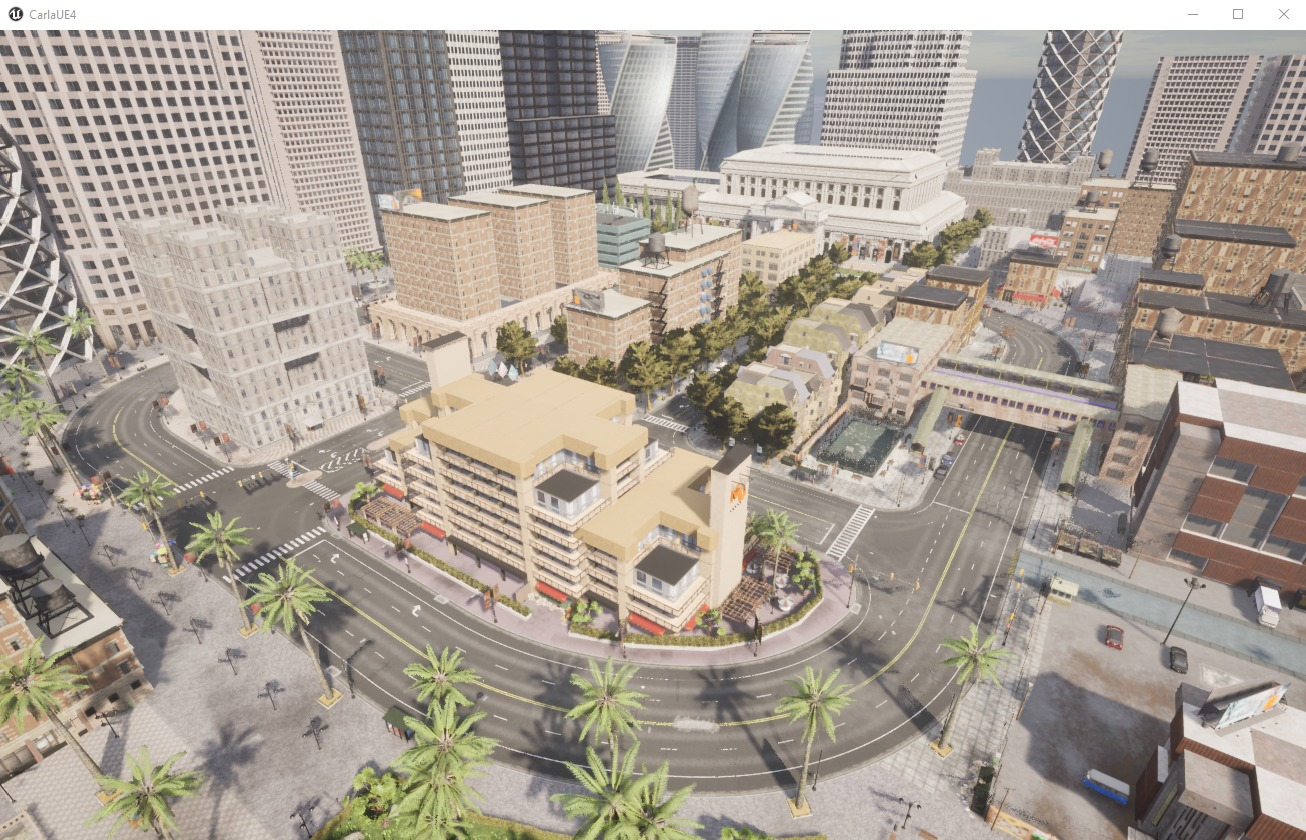
\includegraphics[scale=0.25]{figuras/mapa1-carla.jpeg}
    \captionsetup{justification=centering}
  \vspace{-0.2cm}
     \\\textbf{\footnotesize Fonte: Elaborado pelos autores}
    \label{fig:cidade_carla_simulator_primeira_pessoa}

\end{figure}


As imagens utilizadas no treinamento da IA foram obtidas pelo \textit{sensor camera rgb} fornecido pelo CARLA, que funciona como uma câmera normal capturando as fotos da cena onde o veículo está localizado. A velocidade em que o sensor captura os dados pode ser definida pelo \textit{sensor tick}, sendo que foi adotado um padrão com o atraso mínimo permitido para obter os dados o mais rápido possível.

Utilizando o \textit{sensor lidar ray cast} que simula um sensor LIDAR rotativo de projeção de raios de luz, é possível gerar uma nuvem de pontos da superfície externa de um objeto que, ao final, pode ser utilizado para detectar a distância que o objeto se encontra.

O sensor \textit{camera semantic segmentation} obtém imagens classificando cada objeto com uma cor de acordo com a etiqueta que o elemento recebeu no início da simulação e assim ajudando a definir melhor o que é cada objeto do cenário onde o veículo está localizado, como pode ser observado na Figura \ref{fig:carla_simulator_sensor_segmentacao}.

\begin{figure}[h]
    \centering
    \caption{Visão do sensor de segmentação semântica no CARLA}
    \includegraphics[scale=0.27]{figuras/sensor-seguimentaçao.jpeg}\captionsetup{justification=centering}
  \vspace{-0.2cm}
     \\\textbf{\footnotesize Fonte: Elaborado pelos autores}
    \label{fig:carla_simulator_sensor_segmentacao}
\end{figure}

Ainda sobre sensores, foi utilizado o \textit{sensor other collision} que registra um evento, sempre que há uma colisão com um ator dentro do ambiente do CARLA. Para processar e tratar as imagens obtidas, foi utilizado a biblioteca \textit{OpenCV}, responsável pelos algoritmos de visão computacional fornecendo os dados para a Inteligência Artificial que foi construída com ajuda da ferramenta \textit{Pytorch}, que trata os dados para a tomada de decisões, refletindo na direção dentro do CARLA.

% sobre sensor.camera.rgb
% sensor.other.collision
% =================== Sensores ===================
% ['sensor.camera.rgb', cc.Raw, 'Camera RGB'],
% ['sensor.camera.depth', cc.Raw, 'Camera Depth (Raw)'],
% ['sensor.camera.semantic_segmentation', cc.Raw, 'Camera Semantic Segmentation (Raw)'],
% ['sensor.lidar.ray_cast', None, 'Lidar (Ray-Cast)']]


O simulador CARLA, embora seja estável e bem elaborado, apresenta limitações na criação de cenários complexos, como vias com muitos carros ou a presença de pedestres em determinados momentos. Para superar essas limitações e construir cenários adversos para treinar veículos autônomos, foi recorrido à iniciativa de código aberto denominada ANTI-CARLA \cite{ramakrishna2022anticarla}. Esta ferramenta, é mencionada pelos autores em seu artigo como uma estrutura de testes adversa em CARLA para sistemas de direção autônoma, permitindo a simulação de condições climáticas extremas, variações na luminosidade e outros desafios que podem ser encontrados nas ruas.

\subsection{Método}

Nesta subseção, é apresentado o método para o estudo, desenvolvimento e análise do copiloto de situações adversas e seus resultados. A Figura \ref{fig:metodologia_tcc} ilustra a divisão do trabalho, que consistiu em quatro etapas: investigação sobre o tema, desenvolvimento do copiloto, experimento e coleta de dados e análise dos resultados.

\begin{figure}[H]
    \centering
    \caption{Método de Trabalho}
    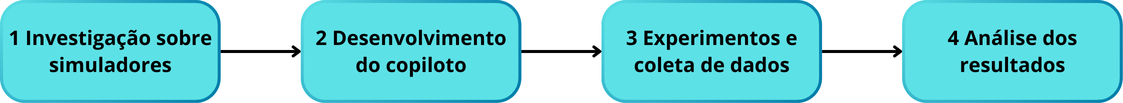
\includegraphics[scale=0.55]{figuras/Metodologia TCC.png}\captionsetup{justification=centering}
  \vspace{-0.2cm}
     \\\textbf{\footnotesize Fonte: Elaborado pelos autores}
    \label{fig:metodologia_tcc}
\end{figure}

Inicialmente, foi conduzido um estudo bibliográfico com o propósito de examinar a utilização de direção de veículos autônomos em simuladores e compreender a efetividade do seu uso para treinamento e direção de veículos em um cenário controlado. Durante essa fase, foi possível observar que existem simuladores que estão munidos com as principais ferramentas e sensores, e, além disso, possuem constantes atualizações, o que contribui com o avanço da tecnologia de direção autônoma, resultando em notáveis transformações.

Em decorrência da realização dos treinamentos, para avaliar o desenvolvimento da solução, foi necessária a busca de simuladores que pudessem auxiliar, tanto na execução, quanto demonstração das evoluções do projeto. Conforme apontado por \citeonline{s19030648}, existem diversas soluções genéricas para validação e simulação de um carro autônomo, no entanto, baseado na necessidade de obter semelhança à realidade, sensores funcionais às análises dos cenários desejados, é prudente a busca de simuladores consolidados que possuam as características essenciais ao problema tratado.

Dentre os principais simuladores encontrados, houve uma análise em relação ao AirSim \cite{airsim2017fsr}, na qual se trata de um simulador multiplataforma \textit{open-source}, utilizado para treinamento de drones, carros e outros, tendo suporte à simulações de software e hardware em loop. Foi criado por engenheiros da Microsoft como uma plataforma para pesquisadores de IA experimentarem algoritmos de aprendizado profundo, visão computacional e aprendizado por reforço para carros autônomos.

Outro simulador com um propósito de ensino e pesquisa é o Udacity Self Driving Simulator, desenvolvido pela Udacity, uma organização educacional com fins lucrativos, a fim de complementar seu curso abordando carros autônomos \cite{udacity-sim}. O simulador, utilizando de um ambiente virtual criado com o Unity 3D para coletar os dados capturados por 3 câmeras localizadas no carro, tem como objetivo principal educar os alunos sobre como treinar carros para navegar em estradas. 

Uma outra opção é o Deepdrive \cite{deepdrive}, simulador com suporte a Windows e Linux, que possui interface de desenvolvimento utilizando da API do Gym, uma biblioteca Python de \textit{open-source} para desenvolver e comparar algoritmos de Aprendizagem por Reforço. Esse simulador oferece sensores GPS, LIDAR e Radar, que podem ser utilizados em um desenvolvimento voltado à veículos autônomos, além de um conjunto robusto de ferramentas de desenvolvimento proporcionadas pelo Unreal Engine, obtendo uma qualidade gráfica extremamente realista e detalhada.

Diante dessas possibilidades, em relação a definição do simulador que seria utilizado, o CARLA é um dos mais competentes para com as necessidades deste trabalho, tendo foco principal na simulação, implementação e execução de algoritmos em veículos autônomos, possuindo suporte abrangente em sensores automotivos e uma comunidade de desenvolvimento ativa.

O CARLA é um simulador de direção autônoma de \textit{open-source} \citeonline{Dosovitskiy17}, criado previamente para ser uma API modular abordando uma série de tarefas envolvendo direção. Inclui ativos digitais como layouts urbanos, edifícios e veículos para criação de mapas, o que amplia mais ainda os escopos para teste. O programa também pode ser usado para comparar o desempenho de três métodos de pipelines modulares de direção autônoma: um modelo treinado usando aprendizado por imitação, um modelo treinado através de aprendizado por reforço e um modelo ensinado através de aprendizado por reforço. Algumas das principais características do CARLA incluem escalabilidade através de uma arquitetura de servidor multi-cliente, um sensor de direção autônoma, uma API flexível, simulação rápida para planejamento e controle, criação de mapas, simulação de cenários de tráfego e bases de direção autônoma.


O uso de simuladores para treinamento de veículos autônomos é crucial para implementar algoritmos de Inteligência Artificial e expô-lo aos mais diversos cenários, resultando em uma melhoria substancial no treinamento em momentos normais e adversos. Dito isso, é importante treinar o modelo em diversas situações cotidianas possíveis vivenciadas por um motorista, bem como a cenários adversos que não podem ser reproduzidos com constância no mundo real. Dessa forma, o uso de uma tecnologia que reproduz o mundo real contribui para um aprimoramento na confiabilidade no algoritmo implementado.

Este artigo busca validar o uso de aprendizado por reforço em veículos autônomos para reagir em situações adversas no simulador CARLA, possibilitando um treinamento extensivo da IA em diversos cenários e tornando o modelo mais preparado para situações adversas. Essa abordagem não só aumenta o preparo dos copilotos existentes, como também melhora a robustez e a confiabilidade dos modelos.

A utilização do simulador no teste e treinamento do modelo de aprendizado por reforço é crucial, mas não isenta a necessidade de validação no mundo real. Pelo simulador, é apenas possível construir uma aplicação robusta e confiável e reduzir o tempo de treinamento, além de possibilitar o treinamento em cenários adversos. Outro benefício é a possibilidade de reproduzir problemas encontrados e a facilidade na otimização do treinamento, garantindo um produto de alta responsividade e eficiência para validar a viabilidade de veículos autônomos.

Na segunda parte do estudo, foi utilizado os cenários de trânsito disponibilizados pelo ANTI-CARLA para automatizar a criação dos ambientes e automação dos testes. Para a criação de um cenário é necessário definir os parâmetros referente a densidade de trânsito, rota e condições climáticas. Posto isso, foi construído um ambiente controlável e replicável para validação do algorítimo. O próximo passo foi a escolha com base nos estudo apresentado por \citeonline{10189852} do agente copiloto \textit{Learning by Cheating} (LBC) para validação das suas capacidades de conclusão das rotas propostas.

% =========== Coletar dados ============= tom 

Os dados coletados durante as execuções foram armazenados para estudo e análise. Desta forma, por meio de boas métricas é possível avaliar o nível confiabilidade do veículo autônomo. As informações coletadas consistem em: colisões do veículo com outros objetos, tempo de reação do veículo, estabilidade de direção, entre outras informações obtidas pelos sensores internos (velocidade e rotação), como já mencionado anteriormente.


% =========== Analisar resultados ============= tom
Na fase de avaliação dos resultados foram analisados os dados coletados e mapeado o  desempenho do veículo ao se manter estável na pista, acurácia do sistema autônomo e a validação de possíveis novos casos que podem ocorrer numa situação real de trânsito.

\section{Experimentos e resultados}
Como resultados preliminares, para avaliar o modelo proposto, foi utilizado o ANTI-CARLA para submeter o copiloto nos cenários de testes adversos no trânsito Figura \ref{fig:nevoa}. Durante o processo de teste foi utilizado um mapeamento de visão com diferentes posições de câmera como entrada para o agente de direção, como exemplificado na Figura \ref{fig:anti-carla}.


\begin{figure}[H]
\caption{Imagens ilustrativas do ANTI-CARLA}
\centering
\begin{subfigure}{0.45\textwidth}
    \centering
    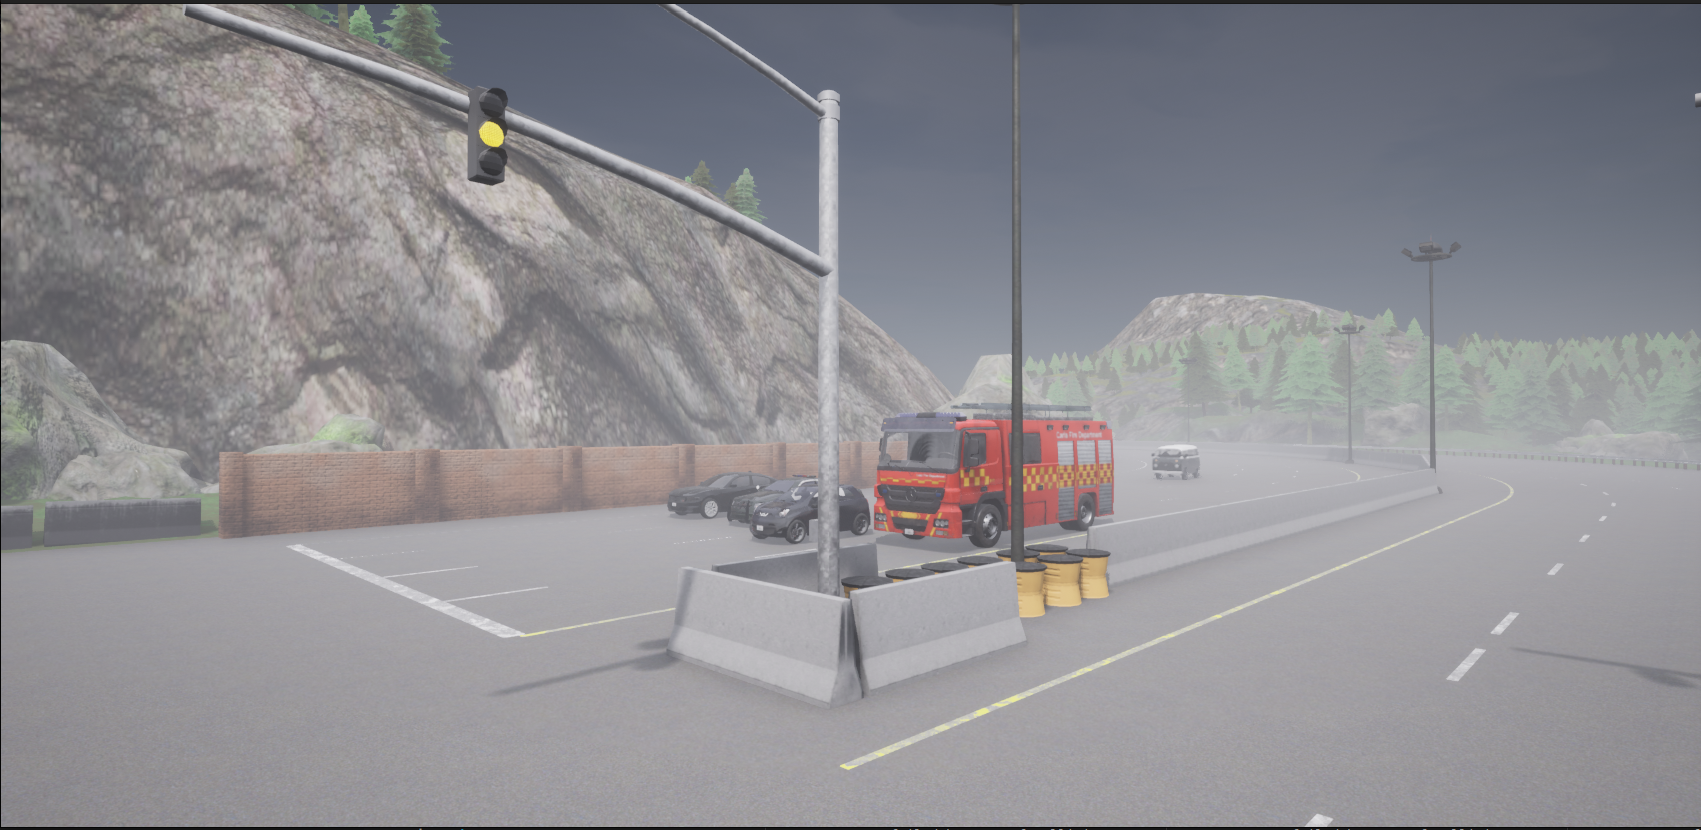
\includegraphics[scale=0.13]{figuras/nevoa.png}
    \captionsetup{justification=centering}
    \caption{ANTI-CARLA em situação de baixa visibilidade}
    \label{fig:nevoa}
    \vspace{-0.2cm}
    \textbf{\footnotesize Fonte: Elaborado pelos autores}
\end{subfigure}
\hfill
\begin{subfigure}{0.45\textwidth}
    \centering
    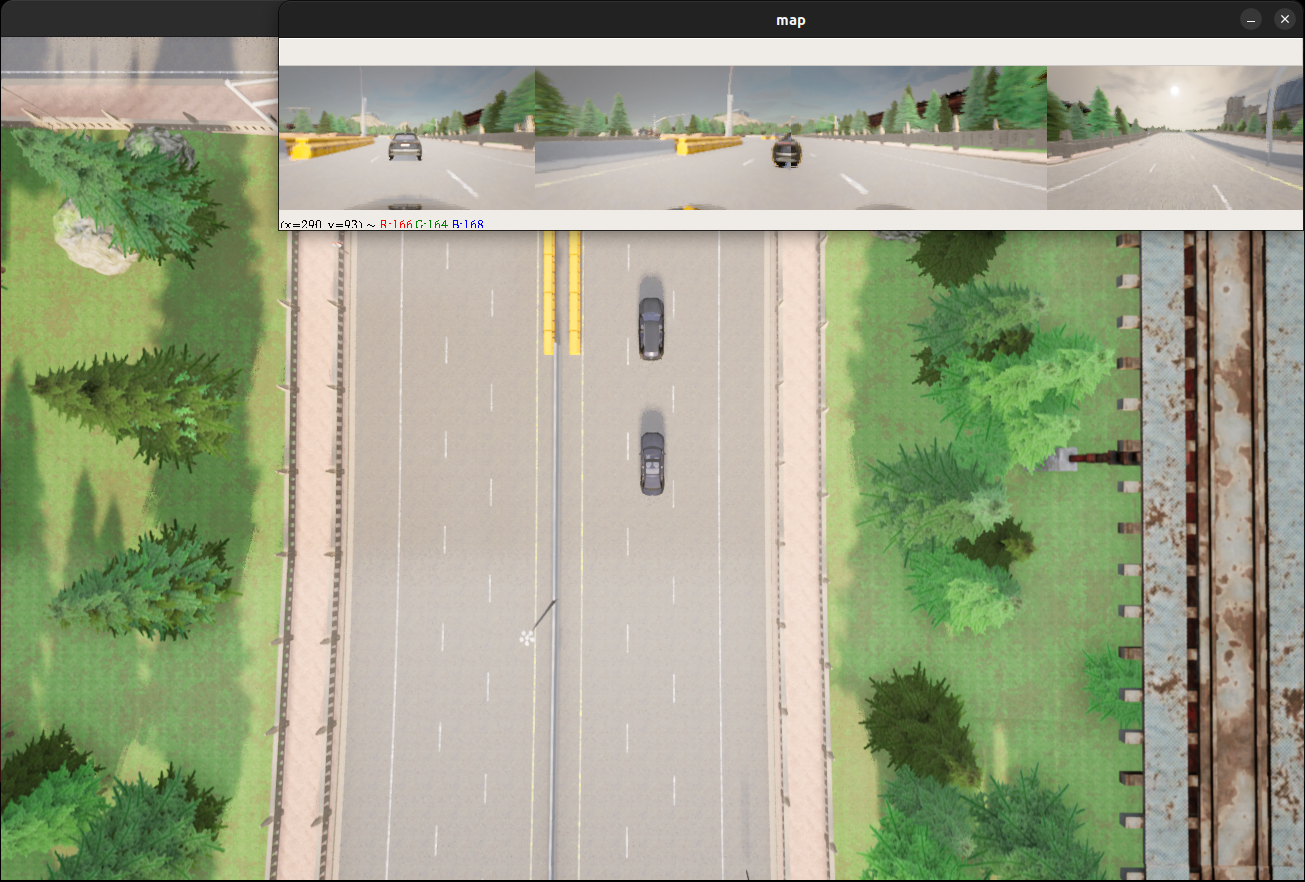
\includegraphics[scale=0.13]{figuras/Anti-carla.png}
    \captionsetup{justification=centering}
    \caption{ANTI-CARLA criando situações de risco}
    \label{fig:anti-carla}
    \vspace{-0.2cm}
    \textbf{\footnotesize Fonte: Elaborado pelos autores}
\end{subfigure}

\end{figure}


Para o copiloto foi utilizado o modelo \textit{Learning by Cheating} (LBC) introduzido por \citeonline{chen2019learning}, que usa o processo de aprendizagem por imitação para o treinamento do agente de direção. Além disso, em cada simulação o agente percorre uma rota do ponto A até o B, onde foram avaliados os seguintes critérios:
\begin{enumerate}
    \item[a)] Porcentagem da rota concluída: É definida pela razão da distância percorrida e a distância total do percurso; 
    
    \item[b)] Porcentagem de extravio da faixa: Essa métrica é calculada pela razão entre a distância total percorrida fora das faixas permitidas e a distância total do percurso concluído. O sistema monitora continuamente a posição do veículo em relação a pontos de referência, chamados de \textit{waypoints}, ao longo da rota. Se a distância entre a posição do veículo e a faixa permitida ultrapassa um limite pré-definido, o veículo é considerado fora da faixa. 
    
    \item[d)] Testes de colisão: A métrica de colisão é calculada com base na contagem de eventos disparados pelo sensor de colisão do CARLA. Cada vez que o veículo colide com um objeto, o sensor gera um evento que é registrado, aumentando a contagem da métrica. O sistema contabiliza colisões com outros veículos, objetos estáticos e pequenas quedas, aplicando filtro para ignorar colisões pequenas ou repetidas com o mesmo objeto;
    
    \item[d)] Tempo Esgotado: A métrica de  tempo esgotado controla um limite de tempo na simulação usando o tempo interno do CARLA. Quando o tempo especificado é alcançado, o status da classe muda para \textit{FALHA}, indicando que o tempo limite foi atingido;

\end{enumerate}

Os critérios foram definidos com a finalidade de avaliar as funções mais básicas do copiloto, principalmente de se manter em uma pista sem colidir até o fim do percurso. Com estas métricas pode-se entender o desempenho do LBC.

Como já definido, o percurso consiste em percorrer de um ponto A do mapa até um ponto B, e é desejado que o veículo complete-o totalmente. Nos casos de teste demonstrados, foram utilizados apenas percursos curtos, como estradas retas sem cruzamentos e com curvas suaves, com a finalidade de focar apenas nas situações adversas.

% ========== como e feito o calculo de extravio da faixa==========

Nos casos de teste, foram consideradas tanto a invasão de faixas erradas quanto a saída para calçadas. Quando detectado um extravio, o sistema acumula a distância percorrida fora da faixa e calcula o percentual correspondente da rota em que o veículo não manteve a direção correta.

% Qual o tempo de timeout da simulacao (Resposta : Pode ser setado no AntiCarla!! parece que cada cenario tem o seu tempo la, mas podem ser alterados)

Para criar os cenários de testes, é possível manipular os eventos e características no mapa da simulação através dos arquivos de configurações do próprio ANTI-CARLA. Os parâmetros são agrupados em 3 itens: 1 - Clima, 2 - Densidade de tráfego e 3 - Densidade de pedestres.


Para manipulação de clima foi ajustado alguns parâmetros como nebulosidade, que varia de 0 a 100, sendo 0 com nenhuma nebulosidade e 100 com a maior quantidade permito pelo CARLA. Além disso foi manipulado a precipitação que também vai de 0 a 100 com a mesma lógica da nebulosidade. Outras características manipuladas foram a densidade do nevoeiro, também variando de 0 a 100, e a distância de visibilidade do nevoeiro de 0 a 100 onde 0 e 0 metros de distancia e 100 são 1000 metros de distância. Para manipular o dia e noite é utilizado o Ângulo de altitude do sol que vai de 0 a 90, onde 0 representa 0° de referencia ao horizonte e 90 é 90°.

A simulação ocorre em 5 cenários diferentes criados pelo próprio ANTI-CARLA, onde foi executado 1 teste para cada cenário em dois tipos de condições:

\begin{enumerate}
    \item[a)] Condições com boa visibilidade (Figuras \ref{fig:boa-1} e \ref{fig:boa-2});
    \item[a)] Condições com baixa visibilidade (Figuras \ref{fig:ruim-1} e \ref{fig:ruim-2});
\end{enumerate}

\begin{figure}[H]
\caption{Imagens do cenário 1 gerada pelo ANTI-CARLA}
\centering
\begin{subfigure}{0.45\textwidth}
    \centering
    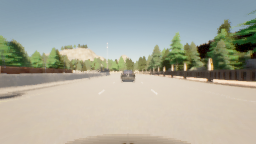
\includegraphics[scale=0.77]{figuras/simulação-boa-1.png}
    \captionsetup{justification=centering}
    \caption{Cenário 1 em boas condições de visibilidade}
    \label{fig:boa-1}
    \vspace{-0.2cm}
    \textbf{\footnotesize Fonte: Elaborado pelos autores}
\end{subfigure}
\hfill
\begin{subfigure}{0.45\textwidth}
    \centering
    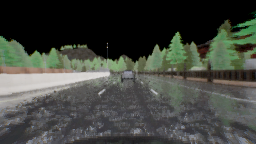
\includegraphics[scale=0.77]{figuras/simulação-ruim-1.png}
    \captionsetup{justification=centering}
    \caption{Cenário 1 em baixas condições de visibilidade}
    \label{fig:ruim-1}
    \vspace{-0.2cm}
    \textbf{\footnotesize Fonte: Elaborado pelos autores}
\end{subfigure}

\end{figure}

\begin{figure}[H]
\caption{Imagens do cenário 2 gerada pelo ANTI-CARLA}
\centering
\label{fig:transito-intenso-motorista}
\begin{subfigure}{0.45\textwidth}
    \centering
    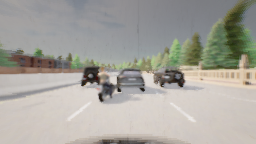
\includegraphics[scale=0.77]{figuras/simulacao-boa-4.png}
    \captionsetup{justification=centering}
    \caption{Cenário 2 em boas condições de visibilidade}
    \label{fig:boa-2}
    \vspace{-0.2cm}
    \textbf{\footnotesize Fonte: Elaborado pelos autores}
\end{subfigure}
\hfill
\begin{subfigure}{0.45\textwidth}
    \centering
    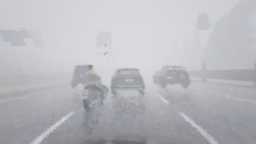
\includegraphics[scale=0.77]{figuras/simulacao-ruim-4.png}
    \captionsetup{justification=centering}
    \caption{Cenário 2 em baixas condições de visibilidade}
    \label{fig:ruim-2}
    \vspace{-0.2cm}
    \textbf{\footnotesize Fonte: Elaborado pelos autores}
\end{subfigure}

\end{figure}

Um dos 5 cenários de trânsito gerado pelo ANTI-CARLA é a inserção de trânsito intenso em uma avenida que pode ser observado nas Figuras \ref{fig:transito-intenso-motorista} e \ref{fig:transito_intenso} :

\begin{figure}[H]
  \centering
  \caption{Simulação de trânsito intenso}
  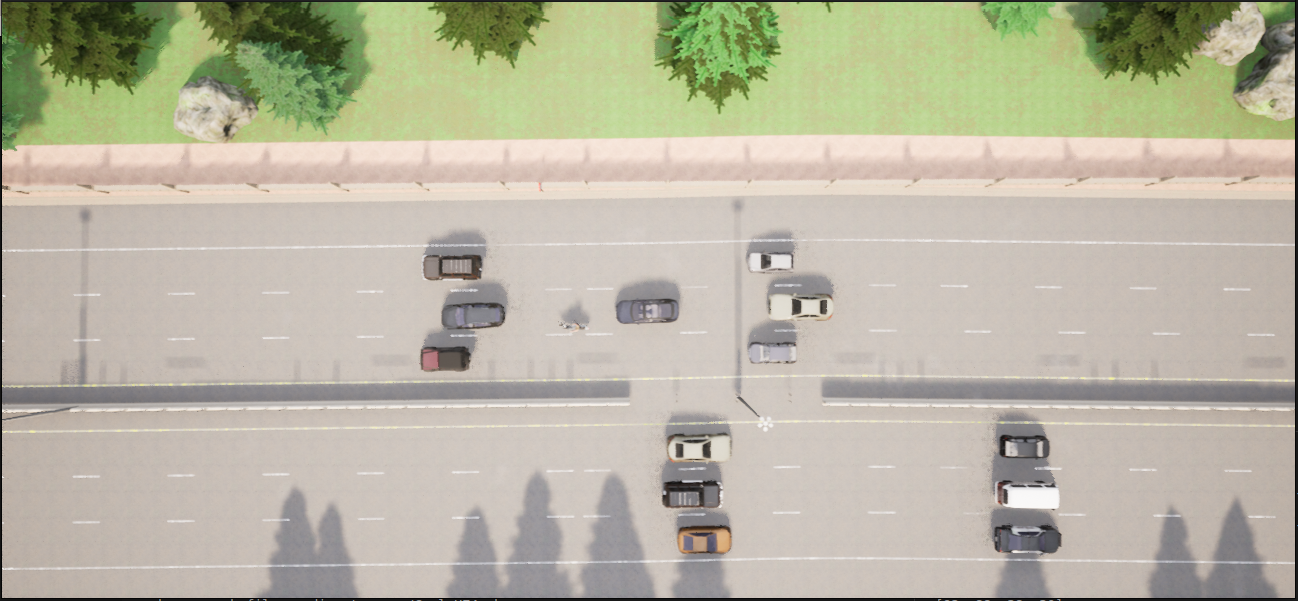
\includegraphics[scale=0.3]{figuras/transito intenso.png}\captionsetup{justification=centering}
\vspace{-0.2cm}
   \\\textbf{\footnotesize Fonte: Elaborado pelos autores}
  \label{fig:transito_intenso}
\end{figure}



O \textit{Learning by Cheating} (LBC) se mostrou eficaz ao lidar com as situações de boa visibilidade, no entanto, em situações adversas foram observadas falhas em vários cenários. Como é possível ver nas Tabelas \ref{tab:Tabela2} e \ref{tab:Tabela3}, o modelo obteve um desempenho satisfatório em cenários de clima favorável.

\begin{table}[H]
\centering
\caption{Tempo de Execução - Condições normais}
\label{tab:Tabela2}
\begin{tabular}{|>{\raggedright\arraybackslash}p{7cm}|>{\raggedright\arraybackslash}p{5cm}|}
    \hline \textbf{Hora de Início} & 2024-06-07 21:02:43 \\
    \hline \textbf{Hora de Término} & 2024-06-07 21:03:28 \\
    \hline \textbf{Duração (Tempo do Sistema)} & 44.51s \\
    \hline \textbf{Duração (Tempo de Simulação)} & 32.7s \\
    \hline \textbf{Razão (Tempo do Sistema / Tempo de Simulação)} & 0.735 \\
    \hline
\end{tabular}
\end{table}
\vspace{0.5cm}

\begin{table}[H]
\centering
\caption{Resultados dos Testes de Critério - Condições normais}
\label{tab:Tabela3}
\begin{tabular}{|>{\raggedright\arraybackslash}p{7cm}|>{\raggedright\arraybackslash}p{3cm}|>{\raggedright\arraybackslash}p{2cm}|}
    \hline \textbf{Critério} & \textbf{Resultado} & \textbf{Valor} \\
    \hline Teste de Conclusão de Rota & SUCESSO & 100 \% \\
    \hline Teste de Rota Fora da Faixa & SUCESSO & 0 \% \\
    \hline Teste de Colisão & SUCESSO & 0 vezes \\
    \hline Tempo Esgotado & SUCESSO & \\
    \hline
\end{tabular}
\end{table}

Ao submeter o algoritmo às situações adversas foram obtidos resultados com uma eficiência variável e pouco satisfatória. As Tabelas \ref{tab:Tabela4} e \ref{tab:Tabela5} contém a exposição e avaliação dos mesmos critérios, desta vez em condições de baixa visibilidade. 

\begin{table}[H]
\centering
\caption{Tempo de Execução - Condições adversas}
\label{tab:Tabela4}
\begin{tabular}{|>{\raggedright\arraybackslash}p{7cm}|>{\raggedright\arraybackslash}p{5cm}|}
    \hline \textbf{Hora de Início} & 2024-06-12 23:00:03 \\
    \hline \textbf{Hora de Término} & 2024-06-12 23:02:38 \\
    \hline \textbf{Duração (Tempo do Sistema)} & 154.82s \\
    \hline \textbf{Duração (Tempo de Simulação)} & 115.05s \\
    \hline \textbf{Razão (Tempo do Sistema / Tempo de Simulação)} & 0.743 \\
    \hline
\end{tabular}
\end{table}

\begin{table}[H]
\centering
\caption{Resultados dos Testes de Critério - Condições adversas}
\label{tab:Tabela5}
\begin{tabular}{|>{\raggedright\arraybackslash}p{7cm}|>{\raggedright\arraybackslash}p{3cm}|>{\raggedright\arraybackslash}p{2cm}|}
    \hline \textbf{Critério} & \textbf{Resultado} & \textbf{Valor} \\
    \hline Teste de Conclusão de Rota & FALHA & 50.35 \%  \\
    \hline Teste de Rota Fora da Faixa & FALHA & 10.15 \% \\
    \hline Teste de Colisão & FALHA & 2 times \\
    \hline Tempo Esgotado & SUCESSO & \\
    \hline
\end{tabular}
\end{table}

% \begin{table}[H]
% \centering
% \caption{Tempo de Execução do Melhor Caso}
% \label{tab:Tabela6}
% \begin{tabular}{|>{\raggedright\arraybackslash}p{7cm}|>{\raggedright\arraybackslash}p{5cm}|}
%     \hline \textbf{Hora de Início} & 2024-06-12 23:02:58 \\
%     \hline \textbf{Hora de Término} & 2024-06-12 23:04:02 \\
%     \hline \textbf{Duração (Tempo do Sistema)} & 64.65s  \\
%     \hline \textbf{Duração (Tempo de Simulação)} & 47.2s \\
%     \hline \textbf{Razão (Tempo do Sistema / Tempo de Simulação)} & 0.73 \\
%     \hline
% \end{tabular}
% \end{table}

% \begin{table}[H]
% \centering
% \caption{Resultados dos Testes de Critério do Melhor Caso}
% \label{tab:Tabela7}
% \begin{tabular}{|>{\raggedright\arraybackslash}p{7cm}|>{\raggedright\arraybackslash}p{3cm}|>{\raggedright\arraybackslash}p{2cm}|}
%     \hline \textbf{Critério} & \textbf{Resultado} & \textbf{Valor} \\
%     \hline Teste de Conclusão de Rota & SUCESSO & 100 \%  \\
%     \hline Teste de Rota Fora da Faixa & SUCESSO & 0 \% \\
%     \hline Teste de Colisão & FALHA & 1 times \\
%     \hline Tempo Esgotado & SUCESSO & \\
%     \hline
% \end{tabular}
% \end{table}

É possível concluir que a variação dos resultados de autonomia do veículo estão diretamente ligadas às condições aplicadas ao cenário. Existe uma incapacidade de tomada de decisão assertiva quando se trata de baixa visibilidade, possivelmente devido ao desempenho insuficiente dos sensores, que podem ser atrapalhados por reflexos, ou pouca amplitude de visualização. A baixa visibilidade compromete a capacidade do sistema de detectar corretamente obstáculos e faixas de rodagem, levando a um aumento no número de falhas, como colisões e desvio de rota. Além disso, a ineficiência no tempo de resposta do sistema em relação às condições ideais reforça a necessidade de aprimoramentos no algoritmo.

Apesar dos cenários disponibilizados pelo ANTI-CARLA serem relativamente simples, como o trânsito em vias movimentadas, foram identificadas algumas dificuldades que o \textit{Learning by Cheating} (LBC) enfrenta quando exposto a diferentes situações. 
Através dos resultados dos testes, é visível que o modelo tem uma boa eficiência nas simulações predefinidas pelo ANTI-CARLA. No entanto, podem ser desenvolvidas melhorias para abranger também as situações adversas supracitadas. 


Como iniciativa para os próximos passos do trabalho, foi realizado um estudo de possíveis algoritmos que podem ser utilizados para auxílio no desenvolvimento do trabalho. Um deles é o de detecção das linhas apresentado por \cite{kim2024carla} para manter o veículo na faixa corretamente. Utilizando algoritmos de reconhecimento de padrão com o auxílio do OpenCV foi possível obter os resultados da Figura \ref{fig:lane-detect3}. 

\begin{figure}[H]
    \centering
    \caption{Detecção das faixas}
    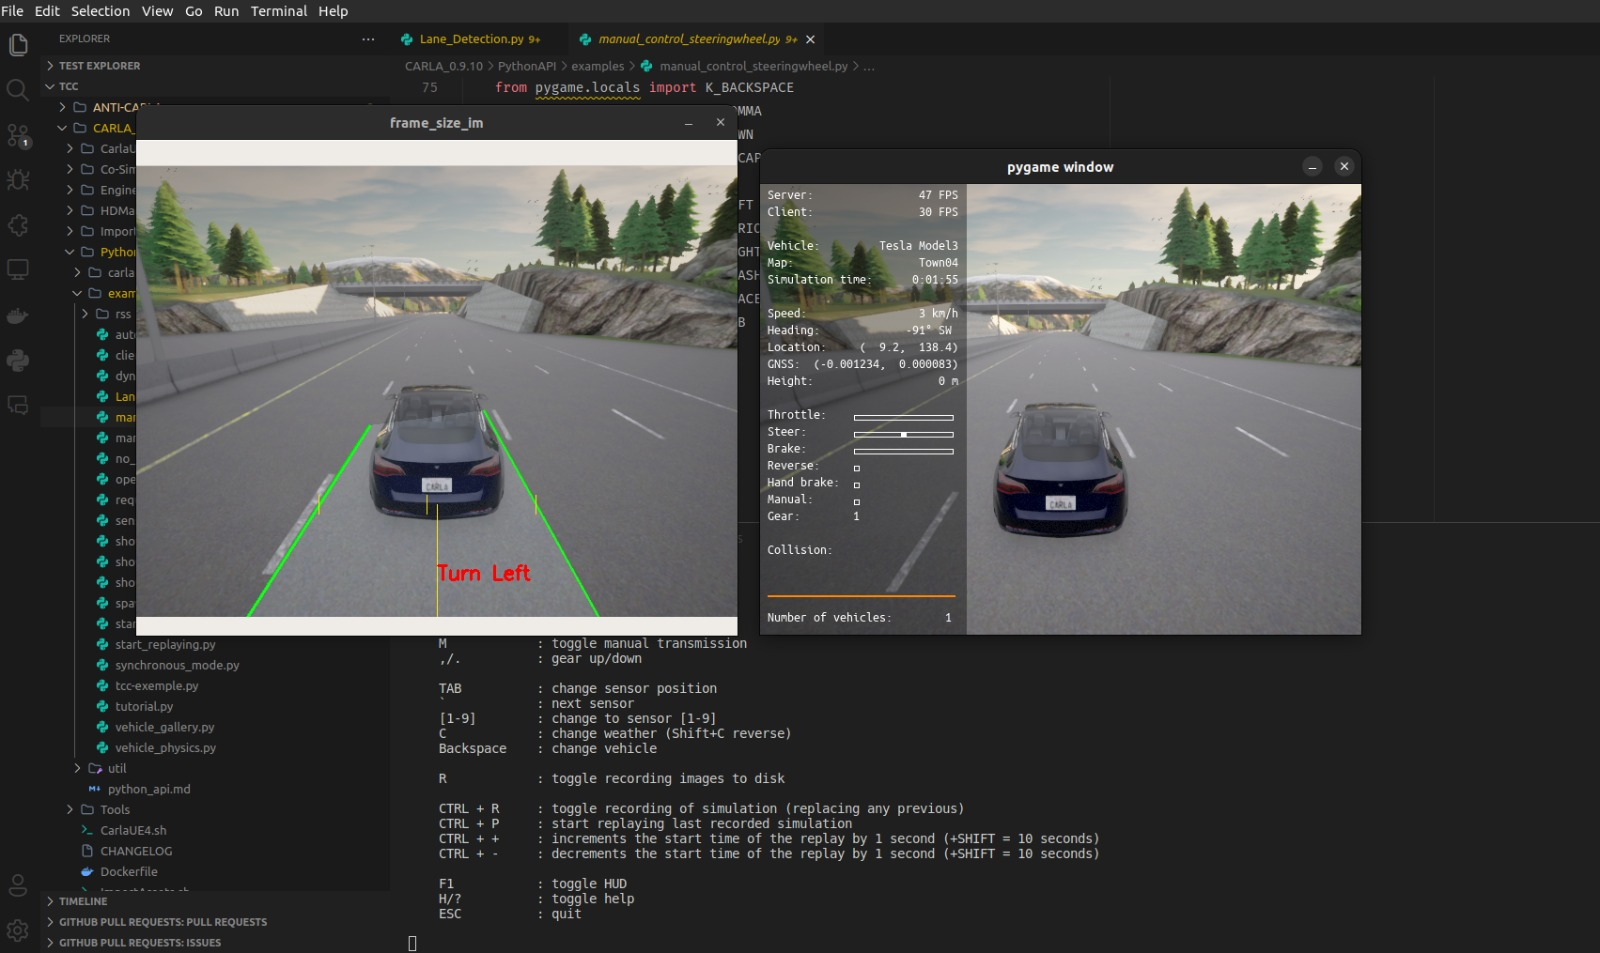
\includegraphics[scale=0.25]{figuras/Lane-detect.jpeg}\captionsetup{justification=centering}
  \vspace{-0.2cm}
     \\\textbf{\footnotesize Fonte: Elaborado pelos autores}
    \label{fig:lane-detect3}
\end{figure}

Os resultados obtidos neste trabalho servirão como base para o desenvolvimento do TCC2, onde será aprimorado o modelo de copiloto para situações adversas, com o objetivo de tornar o veículo autônomo mais seguro e confiável.


\section{Cronograma}

O planejamento para a continuação do desenvolvimento do trabalho durante o segundo semestre de 2024 baseia-se na revisão e continuação dos pontos discutidos no TCC1, como o aprimoramento do modelo de aprendizagem de imitação introduzido pelo \textit{Learning By Cheating} (LBC) para aumentar a precisão na execução de manobras de desvio nos cenários existentes. Além disso, outro requisito importante é a introdução de novos cenários adversos para tornar o modelo mais especializado na tomada de decisão nos mesmos. Em paralelo, novos testes serão implementados e documentados durante o processo como exposto na Figura \ref{fig:cronograma}.

\begin{figure}[H]
    \centering
    \caption{Cronograma TCC 2}
    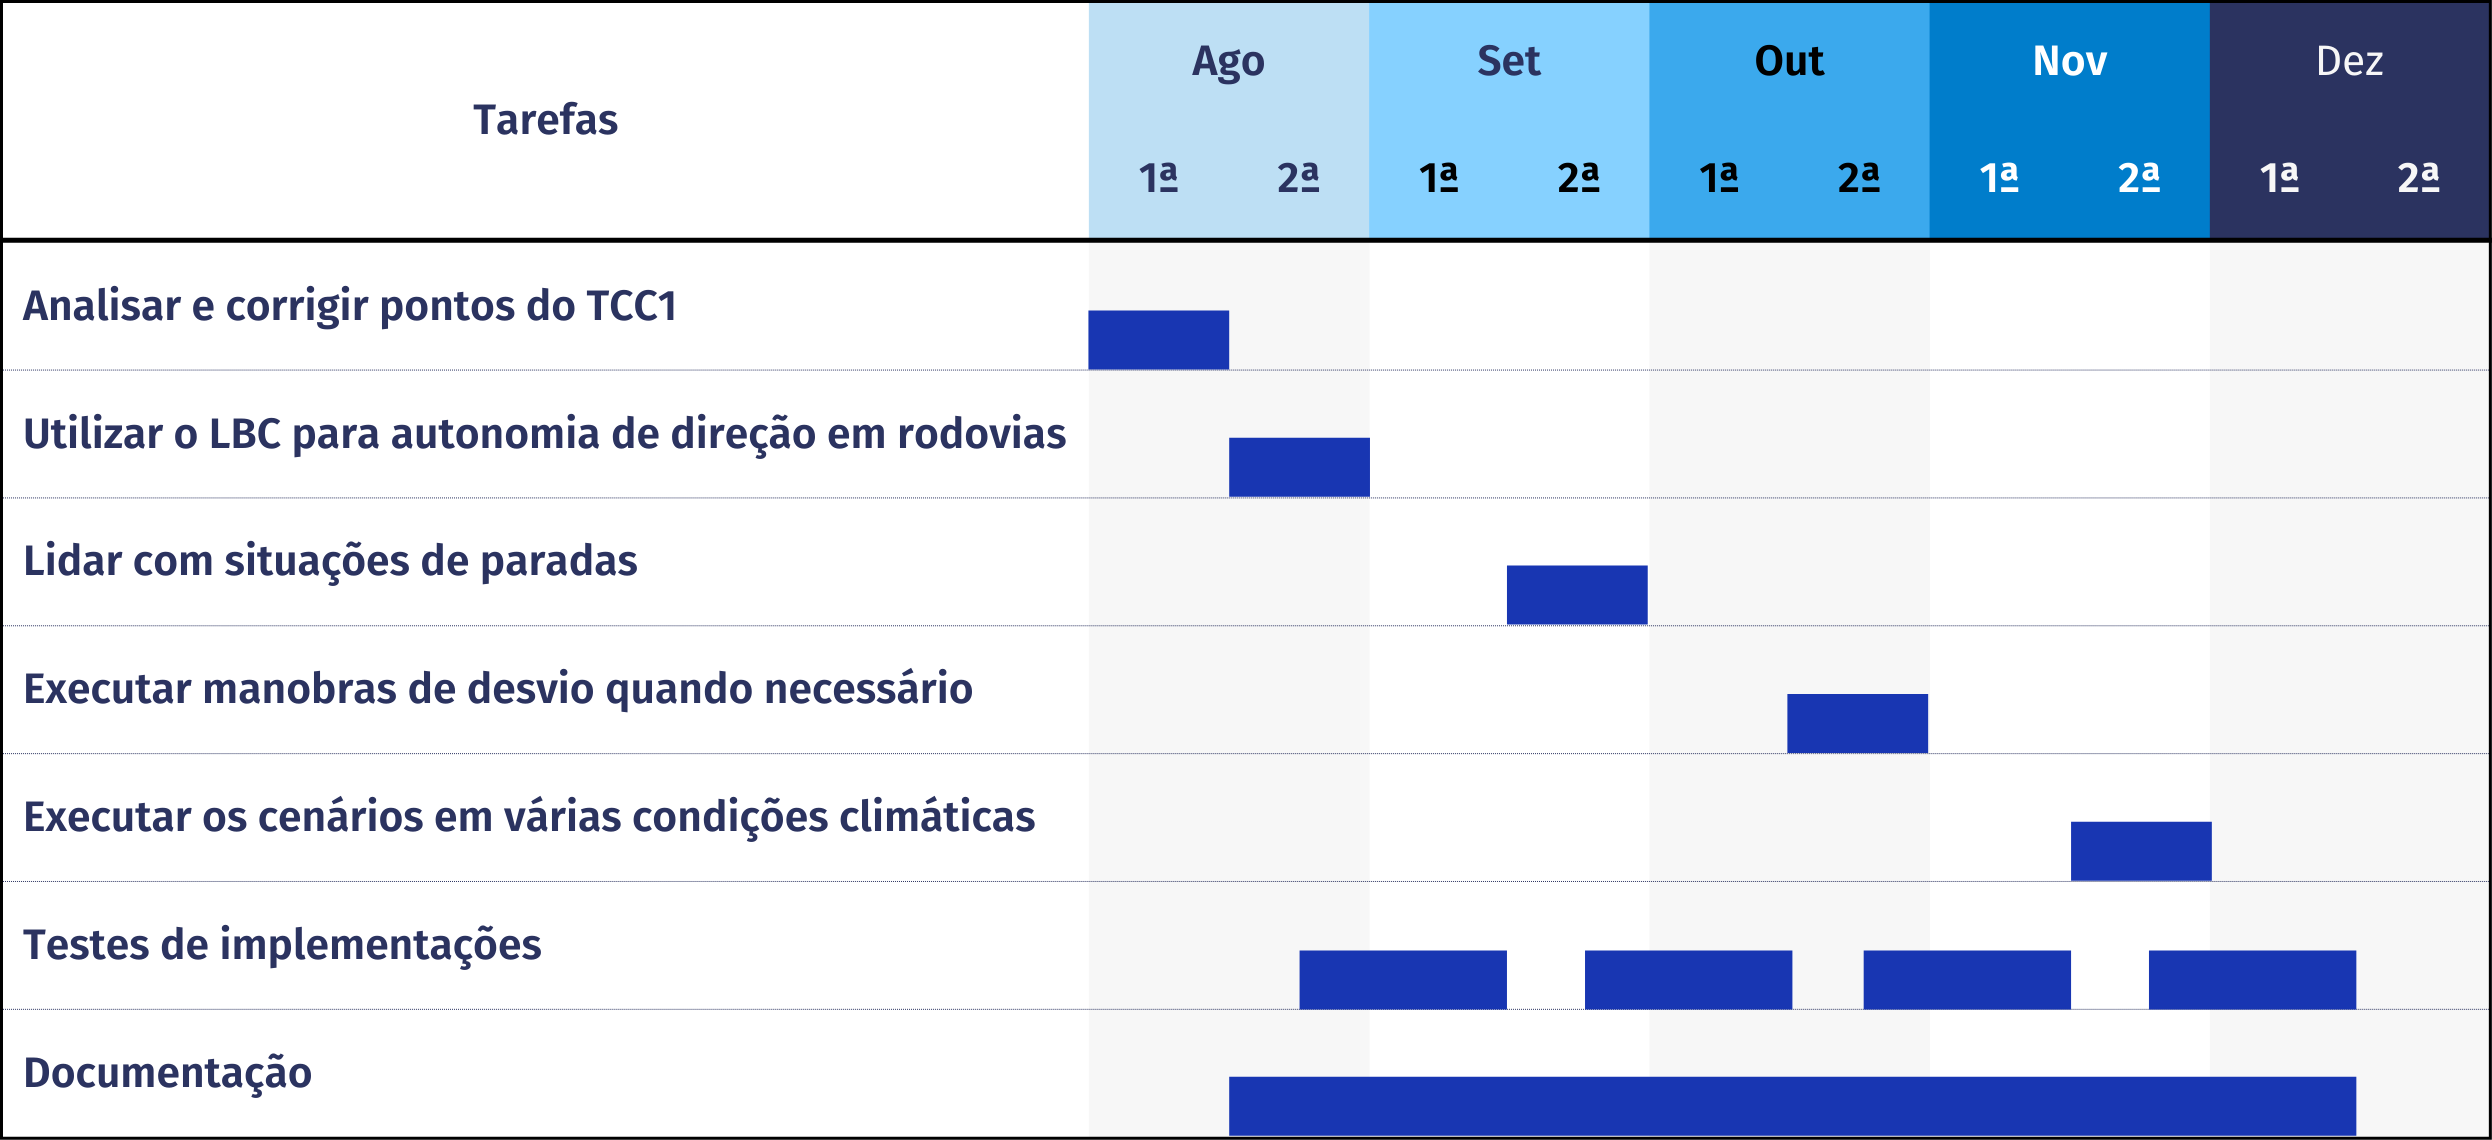
\includegraphics[scale=0.25]{figuras/TCC.png}\captionsetup{justification=centering}
  \vspace{-0.2cm}
     \\\textbf{\footnotesize Fonte: Elaborado pelos autores}
    \label{fig:cronograma}
\end{figure}






% =========== Investigar sobre o assunto ============= fernando

% =========== Construção de um VA demonstrativo ============= fernando
 
 
% ======================= Fernando e tom - Method =======================


% \section{Desenvolvimento}
% \textcolor{red}{Rascunho}

% \section{Experimentos e Resultados Iniciais}
\iffalse
 \newpage
 \singlespace{
 \bibliographystyle{abntex2-alf}
 \bibliography{bibliografia}
 }


\end{document}
\fi
% \cite{9921776} -> fim
% \citeonline{9921776} -> início

%%%%%%%%%%%%%%%%%%%%%%%%%%%%%%%%%%%%%%%%%%%%%%%%%%%%%%%%%%%%%%%%%%%%%%%%%%%%%%%%%%%%%%%%%%%%%%%%%%%%%%%
%%%%%%%%%%%%%% Template de Artigo Adaptado para Trabalho de Diplomação do ICEI %%%%%%%%%%%%%%%%%%%%%%%%
%% codificação UTF-8 - Abntex - Latex -  							     %%
%% Autor:    Fábio Leandro Rodrigues Cordeiro  (fabioleandro@pucminas.br)                            %% 
%% Co-autor: Prof. João Paulo Domingos Silva  e Harison da Silva                                     %%
%% Revisores normas NBR (Padrão PUC Minas): Helenice Rego Cunha e Prof. Theldo Cruz                  %%
%% Versão: 1.0     13 de março 2014                                                                  %%
%%%%%%%%%%%%%%%%%%%%%%%%%%%%%%%%%%%%%%%%%%%%%%%%%%%%%%%%%%%%%%%%%%%%%%%%%%%%%%%%%%%%%%%%%%%%%%%%%%%%%%%
\section{\esp Introdução}

A formatação deverá ter parágrafo recuado a 1,25 centímetros, tamanho 12, fonte Arial ou Times New Roman , espaçamento 1,5 justificado. Todo o texto deverá conter essa formatação com exceção para citações textuais, 
descritas adiante neste modelo. Os títulos dos capítulos devem utilizar a formatação caixa alta, negrito, tamanho 12.

\section{\esp Desenvolvimento}

Todo título de seção ou subseção deverá ser seguido de texto.
Para as seções textuais utilizar numeração progressiva em algarismos arábicos, limitada até a seção quinária 
(NBR 6024/2003) da ABNT. Devem ser diferenciadas utilizando os recursos gráficos abaixo \cite{manualpuc}.
Os títulos das seções primárias devem ser em caixa alta, negrito, tamanho 12.

\subsection{\esp Seção secundária}

Os títulos das seções secundárias terão caixa baixa, negrito, tamanho 12.

\subsubsection{\esp Seção terciária}

Caixa baixa, itálico, negrito, tamanho 12.

\subsubsubsection{\esp Seção quartenária}
 
 Caixa baixa, sublinhado, negrito, tamanho 12.
 
 \subsubsubsubsection{\esp Seção quinária}
 
 Nas seções quinárias, deve ser usado caixa baixa, sem negrito, tamanho 12.

\section{\esp Elementos flutuantes}

Elementos inseridos no texto como imagens, tabelas, algoritmos etc.
Recomenda-se a colocação das ilustrações de forma centralizada, dentro das margens. 
Caso não seja possível, em \citeonline{manualpuc} recomenda-se utilizar recursos como: 
 a) utilizar letras com tamanho menor ao padrão do texto; a) imprimir a ilustração no sentido vertical; 
 c) imprimir em folha A3 ou superior e dobrá-la até atingir o tamanho da folha A4. 

Nas normas da PUC é afirmado a necessidade de se observar que todos os elementos flutuantes inseridos devem ter a formatação básica:

\begin{enumerate} 
 \item [a)] Título centralizado localizado na parte superior; 
 \item [a)] Fonte em tamanho 10 na parte inferior;
 \item [c)] Devem ser inseridas o mais próximos do texto que as referenciam.
\end{enumerate}


\subsection{\esp Inserções de ilustrações}

As ilustrações devem ser inseridas seguindo o exemplo da Figura \ref{fig:figura1}. 
% Figura
\begin{figure}[ht]
	\centering	
	\caption[\hspace{0.1cm}Grade Computacional.]{Uma Grade Computacional como fonte transparente}
	\vspace{-0.4cm}
	\includegraphics[width=0.6\textwidth]{figuras/grade-comp.png}
	% Caption centralizada
% 	\captionsetup{justification=centering}
	% Caption e fonte 
	 \vspace{-0.2cm}
	\\\textbf{\footnotesize Fonte: \cite{cap-livro} }
	\label{fig:figura1}
\end{figure}
\vspace{-0.5cm}

\subsection{\esp Inserção de tela de software}

Nos casos de telas de \textit{software}, devem ser inseridas como figuras, e referenciadas no texto
como na Figura \ref{fig:tela1}. Além disso, é necessário que seja citada no texto a empresa desenvolvedora.

% Figura
\begin{figure}[!ht]
	\centering	
	\caption[\hspace{0.1cm}Exemplo de tela de software.]{Exemplo de tela de software}
	  \vspace{-0.4cm}
	\includegraphics[width=.8\textwidth]{figuras/tela1.png}
	% Caption centralizada
% 	\captionsetup{justification=centering}
	% Caption e fonte
	 \vspace{-0.3cm}
	\\\textbf{\footnotesize Fonte: \cite{tela1}}
	\label{fig:tela1}
\end{figure}

\subsection{\esp Inserção de gráficos e mapas}

O gráfico é um tipo de ilustração que deve conter todos os elementos citados e também a descrição de seu título
diferenciando-o das figuras da mesma forma que no Gráfico 1. 

\begin{center}
	\centering	
 	\textbf{Gráfico 1 - Exemplo de um gráfico} \\
%  	  \vspace{0.cm}
	\includegraphics[width=0.7\textwidth]{figuras/access.png}
	% Caption centralizada
% 	\captionsetup{justification=centering}
	% Caption e fonte
	 \vspace{-0.3cm}
	\\\textbf{\footnotesize Fonte: \cite{tese}}
	\label{grafico1}
\end{center}

A mesma regra se aplica para mapas, que devem ser adicionados seguindo as regras de apresentação já mostradas. No caso específico,
o título e a numeração, também como os gráficos, devem começar do numeral ``1'' depois da marcação ``Mapa'' seguido do nome do elemento.
Exemplo: \textbf{Mapa 1 - Exemplo de um Mapa}.

 \subsection{\esp Tabelas}

As tabelas devem ser abertas nas laterais, com espaços verticais separando
as colunas e sem espaços horizontais, exceto na
separação do cabeçalho. Um exemplo é a Tabela \ref{tab:tabela1}. 

% Tabela
\begin{table}[htb]
	\centering
	\caption{\hspace{0.1cm} Exemplo de uma tabela}
	\vspace{-0.3cm} % espaço entre titulo e tabela
	\label{tab:tabela1}
	% Conteúdo da tabela
	\begin{tabular}{l|c|c}
  \hline
    \textbf{Imagem}	& \textbf{transferência} & \textbf{tempo} \\
    \hline
     estação 1	& 7,72 MB/s &  1:22:18 \\
     estação 2	& 7,72 MB/s &  1:22:17 \\
     estação 3	& 7,59 MB/s & 1:24:25 \\
     estação 4  & 7,53 MB/s & 1:43:27 \\
     estação 5	& 6,14 MB/s  &  1:24:41 \\
     estação 6  &  7,50 MB/s & 1:23:53 \\
     estação 7  & 7,58 MB/s  &  1:24:02 \\
     estação 8  & 7,8 MB/s  &  1:29:06 \\
     estação 9  & 7,9 MB/s  &  1:30:05 \\
     estação 10 & 8,0 MB/s  &  1:32:03 \\
     \hline
 \end{tabular}
 	\vspace{.1cm}  %espaço entre tabela e fonte
	\small
	% Fonte
	{\footnotesize\\ \textbf{Fonte: \cite{monog-fabio}}}
\end{table}

\subsection{\esp Quadros}

Os quadros diferem das tabelas por apresentarem dados textuais.
Esses dados podem ser esquemáticos, comparativos ou descritivos.

   \begin{center}
          \centering
       	\textbf{Quadro 1 - Bandas/Artistas de Rock e outros}\\
% 	\vspace{-0.3cm} % espaço entre titulo e tabela
        \label{quadro1}
	\begin{tabular}{|c|c|c|c|} \hline
	\multicolumn{4}{|c|}{\textbf{Bandas ou Artigas de Rock e outros}} 	  \\ 
		\hline \textbf{	Progressivo} & Pink Floyd & Jethro Tull	& Yesterday \\ 
		 \hline \textbf{ Metal}  & Metallica & Iron Maidam & Black Sabath \\ 
		\hline \textbf{	Arena Rock} & Led Zeppelin & The Rolling Stones & Beatles \\ 
		\hline \textbf{ Punk} & Ramones & Black Flag & NOFX	\\ 
		\hline \textbf{	Nacional} & Ira & Engenheiros & Vinil	\\ 
		\hline \textbf{	S.J.E.} & Apolo XI & Invasão 7 & Por do Sol \\ 
		\hline \textbf{	Grunge} & Nirvana & Pear Jam & Alice in Chains	\\ 
		\hline \textbf{	Rock Folk} & Bod Dylan & The Byrds &  The Mamas \& the Papas \\
		\hline \textbf{	Blues} & B.B. King & Albert Colins & Mady Wathers \\ 
		\hline \textbf{	New Wave} & The Police & The Pretenders, &  Duran Duran\\ 
 		\hline \textbf{	Rock Folk} & Bod Dylan & The Byrds &  The Mamas \& the Papas \\
 		\hline \textbf{	Rock alternativo} & R.E.M.& Hüsker Dü & Big Black\\ 
 		
		\hline
	\end{tabular}
	\vspace{0.1cm} 
	{\footnotesize\\ \textbf{Fonte: Dados da pesquisa}}
   \end{center}

Para gráficos, quadros e tabelas, cujos dados foram extraídos da própria pesquisa, 
 usar a expressão: Dados da pesquisa. Ver exemplo no Quadro 1.
   

\subsection{\esp Inserção de algoritmos}

Para inserir um algoritmo, utilizar o exemplo do Algoritmo  \ref{alg:rnagenerica}.
Todos os algoritmos devem ser inseridos como figura, indicada por nome e  fonte. Caso 
forem de própria autoria, isso deverá ser mencionado na fonte, como elaboração feita pelos autores.

% algoritmo
% \begin{figure}[ht]
\begin{center}	
	% Arquivo da figura
% 	\caption[\hspace{0.1cm} Texto da figuras.]{Algorítmo CAC RD Neural}
         \textbf{Algoritmo 1 -  CAC RD Neural}
	\vspace{-0.3cm}
\begin{minipage}[ht]{13cm}
\begin{algorithm}[H]
  \footnotesize
  \caption{CAC-RD Neural}
  \label{alg:rnagenerica}
  \begin{algorithmic}[1]
      \STATE \textbf{Entrada:} Requisição da chamada
    \STATE \textbf{Saída:} Aceitação ou bloqueio da solicitação
    
    \STATE Preenche o vetor de $attributes.size+1$ atributos com os valores dos atributos, sendo a primeira posição do vetor preenchida com o valor 1
		\STATE $hidden\_layer\_size =  attributes.size*2+1;$

    \FOR{$i$ = 1 to $attributes.size+1$}
    	\STATE \textbf{normalizar}($Entrada_i$)
    \ENDFOR

		\STATE $double [] net = new double [hidden\_layer\_size];$
    \STATE $net = hidden\_layer\_weights * attributes;$
   	\FOR{$i$ = 0 to hidden\_layer\_size}
			\STATE $net [i] = 1.0 / (1.0 + exp((-1.0)*net[i]));$
		\ENDFOR

		\STATE $double [] ipVector = new double [hidden\_layer\_size+1];$
    \STATE $ipVector [0] = 1.0;$
   	\FOR{$i$ = 1 to $hidden\_layer\_size+1$}
			\STATE $ipVector [i] = net [i-1];$
		\ENDFOR
		
		\STATE $output = output\_layer\_weights *  ipVector;$
    \STATE output = \textbf{desnormalizar}(Saída)
    \STATE \textbf{net\_update} (requisition);
    
    \STATE \textbf{Retorna} output; FIM
  \end{algorithmic}
\end{algorithm}
% \vspace{-0.3cm} % espaço entre algoritmo e fonte

\small \centering \textbf{\footnotesize Fonte: \cite{mestrado}.}
\end{minipage}
\end{center}
% \end{figure}

Para ilustrações criadas ou adaptadas a partir de outras ilustrações, usar as expressões: 
“Adaptado de...” ou “Criado pelo autor`` com dados extraídos de \ldots
   
   
\section{\esp CITAÇÕES}


Referências deverão ser adicionadas no arquivo \textit{bibliografia.bib}. Cada referência deverá ser adicionada conforme o padrão de normalização da PUC, 
o qual poderá ser consultado na página da biblioteca da PUC Minas \cite{manualpuc}. Todas as publicações citadas no texto deverão ter correspondente nas referências, 
e as indicações de autoria da citação e do ano deverão ser idênticas aos dados expostos.


\subsection{\esp Citação livre ou indireta}

Quando se reproduzir ideias, sem transcrever as palavras do autor, a indicação da página é opcional. Exemplos desse tipo de citação:
\begin{enumerate} 
 \item [a)] Citação com um autor \cite{knuth}. 
 \item [b)] Citação de artigos em revistas com dois autores \cite{artigo01}.
  \item [c)] Trabalho em congresso com três autores \cite{dovzan:01}.
 \item [d)] Trabalhos com mais de três autores \cite{cap-livro}.
 \item [e)] Dois autores em duas obras distintas \cite{knuth,groupp}.
 \item [d)] Trabalhos distintos com vários autores \cite{congresso,cap-livro}.
 
\end{enumerate}

\subsection{\esp Citação direta ou textual}

Transcrição literal de textos de outros autores. Nesse caso, deverão ser especificadas as páginas consultadas. 
Se desejar, poderão ser grafadas em itálico para melhor visualização.

\subsubsection{\esp Textual Curtas}

Quando curtas (até 3 linhas) serão inseridas na sequência normal do texto, entre aspas com as mesma formatação.

\subsubsection{\esp Textual Longas}

Citações longas (mais de 3 linhas) deverão constituir um parágrafo independente, recuado a 4 cm da margem esquerda, 
com letra tamanho 10 e digitado em espaço simples, sem aspas.
\begin{citacaodireta}
Hegel chama trabalho à forma específica da satisfação das necessidades, que
distingue da natureza o espírito existente. Assim como a linguagem infringe
a imposição da intuição e ordena o caos das múltiplas sensações em coisas
identificáveis, assim o trabalho infringe a imposição do \hspace{0.1cm}desejo \hspace{0.1cm}imediato \hspace{0.1cm}e
suspende, por assim dizer, o processo de satisfação das necessidades.
\cite[25]{habermas}.
\end{citacaodireta}


% Artigo \cite{whatershed:01}

\subsubsection{\esp Textual de outros idiomas (Tradução)}

\begin{citacaodireta} 
Um \textit{cluster} é um computador paralelo construído de componentes e processos de \textit{software} (tal como sistema de \textit{software}). 
Um \textit{cluster} é formado de nós, cada um contendo um ou mais processadores, memória que é compartilhada por todos os processadores do nodo 
(somente eles), e dispositivos periféricos adicionais (tais como discos), conectados pela rede e que permitem tráfego de dados entre os nós...
\cite[p. 10, tradução nossa]{groupp}\footnote {  … a cluster is a parallel computer that is constructed of commodity  componets and runs 
(as its system software) commodity software. A cluster is made of nodes, each conteining one or more processors, memory that is  shared 
by all of the processors in (and only on) the node, and addtional peripheral devices (surch as disks),
 connected by network that allows data to move between the nodes}.
\end{citacaodireta}
 
\subsection{\esp Exemplos de citações} 

Alguns exemplos de citações mais utilizadas e/ou que geram algumas dúvidas. É válido observar que não citaremos
todas as possibilidades de citações da norma da PUC Minas, sendo assim é de extrema relevância que se consulte 
o documento no site da Biblioteca da PUC Minas para maiores esclarecimentos acerca de citações \cite{manualpuc}.

\subsubsection{\esp Citação de monografia, dissertação e tese}

Exemplo de citação de monografia de curso de graduação ou especialização pode ser vista em \citeonline{monog-fabio}.
Exemplo de dissertação de mestrado é referida como \citeonline{mestrado}.

Para o caso de doutorado é citado da seguinte forma, Góes (\citeyear{tese}). Nesse exemplo é válido observar a forma
como está escrito no documento \LaTeX, pois citações que compreendem no texto o nome do autor como sua parte, necessitam 
do parâmetro \verb$\citeonline{}$. 

\subsubsection{\esp Livros e partes de livros}

Exemplo de capítulo de livro fica conforme este exemplo \cite{cap-livro}.

Para livros citados no corpo do texto e com duas citações juntas, ver os exemplos \citeonline{knuth,groupp}.
Caso essa citação não fizesse parte do texto será referencia dessa forma \cite{knuth,groupp}.

Citações institucionais ou documentos técnicos de alguma entidade devem ser citados desta forma \cite{pmbok}.

\subsubsection{\esp Tela de software}

Para  citar a tela de um \textit{software} faça da seguinte forma, \citeonline{tela1}.

\subsubsection{\esp Citações da Biblia Sagrada}

A Bíblia está dividida em duas grandes partes: O Antigo Testamento e o Novo Testamento, divididos em livros, capítulos e versículos. 
Portanto, a citação de partes da Bíblia deve apresentar o título do livro de forma abreviada ou por extenso, o número do capítulo e o número do versículo.


\begin{citacaodireta}
Moisés estendeu a mão sobre o mar. Com um forte \hspace{-0.1cm} vento \hspace{0.1cm} leste a \hspace{0.1cm}sobrar a
noite toda, o Senhor repeliu o mar e o pôs a seco. As águas se fenderam e
os filhos de Israel entraram no meio do mar a pé enxuto, enquanto as águas
formavam uma muralha à direita e à esquerda deles (\citeauthor{biblia} 14,21).
\end{citacaodireta}

\subsection{\esp Conclusão}

Discussão dos resultados obtidos na pesquisa. É onde se colocam as observações do autor. 
Poderá também apresentar sugestões de novas linhas de estudo.

A conclusão deve estar de acordo com os objetivos do trabalho.

A conclusão não deve apresentar citações ou interpretações de outros autores.

% \subsection{\esp Trabalhos futuros}
% 
% Sugestões de estudos posteriores são ser adicionados subseção deste capítulo de conclusão.

%%%%%%%%%%%%%%%%%%%%%%%%%%%%%%%%%%%
%% FIM DO TEXTO
%%%%%%%%%%%%%%%%%%%%%%%%%%%%%%%%%%%

% \selectlanguage{brazil}
%%%%%%%%%%%%%%%%%%%%%%%%%%%%%%%%%%%
%% Inicio bibliografia
%%%%%%%%%%%%%%%%%%%%%%%%%%%%%%%%%%%

 \newpage
 \singlespace{
 %\bibliographystyle{abntex2-alf}
 \bibliography{bibliografia}
 }

\end{document}
